% =====================================================================
% Paper 12 - NIST 800-53 as Code: Quantifying the Compliance-Exposure
% Reduction of Continuous Automated Evidence Collection and Its
% Automatability Ceiling. IEEE TNSM submission. Build with tectonic.
% Reproducibility: results/primary_v1/ (25 seeds, frozen on 800-824).
% Run src/run_evaluation.py.
% =====================================================================
\documentclass[journal]{IEEEtran}

\usepackage{graphicx}
\usepackage{adjustbox}
\usepackage{booktabs}
\usepackage{amsmath}
\usepackage{amssymb}
\usepackage{newtxtext,newtxmath}
\usepackage{hyperref}
\usepackage{xurl}
\usepackage{url}
\usepackage{array}

\graphicspath{{figures/}}

\title{NIST 800-53 as Code: Quantifying the Compliance-Exposure Reduction of\\
Continuous Automated Evidence Collection and Its Automatability Ceiling}

\author{%
  \IEEEauthorblockN{Harshavardhan Malla}
  \IEEEauthorblockA{Independent Researcher}%
}

\renewcommand{\textendash}{-}
\renewcommand{\textemdash}{-}
\usepackage{etoolbox}
\makeatletter
\patchcmd{\abstract}{---}{:\space}{}{}
\patchcmd{\IEEEkeywords}{---}{:\space}{}{}
\makeatother
\begin{document}
\maketitle

\begin{abstract}
Federal systems must show that their security controls remain effective over time, not only at an
annual audit. Continuous monitoring guidance and machine-readable control formats make it possible
to collect control evidence automatically and continuously, so a control that drifts out of
compliance is caught in days rather than at the next assessment. The operational question is how
large that benefit is, and what bounds it. We answer with a pre-registered simulation of a
200-control catalog drifting as a Poisson process over two years, with hypotheses, thresholds, and
evaluation seeds locked before any result was inspected. On automatable controls, continuous
monitoring cuts the mean time to detect drift from 272 days under annual assessment to 1 day, a
factor of 272 (95\% bias-corrected and accelerated bootstrap interval $[269, 275]$). The overall
exposure reduction is bounded by automatability: continuous monitoring removes 0.567 of annual
exposure ($[0.553, 0.581]$) against a ceiling of 0.643 ($[0.628, 0.660]$) set by the
automatable-exposure share, because the controls a machine cannot check form a floor that no
detection speed can lower. The benefit shows diminishing returns as the manual cadence tightens
(33{,}000 control-days saved over annual but 16{,}000 over quarterly) and concentrates in
high-drift controls: the top-drift quartile alone captures 79\% of the achievable reduction.
We also derive these findings in closed form. A short exposure decomposition shows that the
fractional reduction is bounded above by the automatable-exposure share, $R \le C$, that the absolute
benefit must diminish as the manual cadence tightens, and that a heavy-tailed drift distribution
forces the benefit to concentrate, with the closed form reproducing the frozen ceiling $C = 0.643$
and realized reduction $R = 0.567$. The deployment rule that follows is concrete. Instrument the
high-drift automatable controls first, size programmatic expectations to the automatable-exposure
share rather than to detection latency, and treat the manual remainder as an irreducible residual.
\end{abstract}

\begin{IEEEkeywords}
continuous monitoring, NIST 800-53, compliance automation, OSCAL, policy as code, control drift,
compliance exposure, pre-registration, reproducibility
\end{IEEEkeywords}

\section{Introduction}
\IEEEPARstart{A}{federal} authorization to operate rests on a body of security
controls~\cite{nist80053}, and that authorization is a statement about a moment in time. The
controls are assessed, the system is judged acceptable, and an authorizing official signs. Between
that signature and the next assessment, the system keeps running and its configuration keeps
changing. A control drifts out of compliance when an audit log is silently disabled, a TLS
certificate expires, a firewall rule is loosened for a troubleshooting session and never restored,
or a baseline configuration is edited by hand. Each such drift opens a window of exposure that
lasts until someone notices. Under the traditional model of periodic assessment, noticing happens
at the next audit, which for many control families is a year away.

Information security continuous monitoring~\cite{nist80137} was introduced precisely to shorten
that window. Its assessment companion~\cite{nist80137a} frames continuous monitoring as an ongoing
program rather than a periodic event, and the Open Security Controls Assessment
Language~\cite{oscal} gives the controls a machine-readable representation so that evidence can be
collected, checked, and compared by software. Together these enable a compliance-as-code posture:
a control is expressed as a checkable rule, the rule is evaluated on a short cadence, and a drift
is caught within that cadence rather than at the next periodic assessment. The policy-as-code
tooling that the wider industry has converged on, from general policy engines~\cite{opa} to
desired-state configuration systems~\cite{powershelldsc}, makes the mechanics routine for the
controls that can be expressed this way.

The promise is attractive enough that it is easy to overstate. Two facts bound it. First, not
every control is machine-checkable. A control that requires a documented and approved policy, a
signed agreement, or a physical-security inspection still demands human assessment; continuous
collection cannot reach it, so it stays on the periodic cadence no matter how fast the automatable
controls are checked. The un-automatable remainder therefore sets a floor on the achievable
reduction in exposure. Second, exposure is not spread evenly across the catalog. A control that
drifts twice a decade contributes little exposure whatever the monitoring regime, while a control
that drifts monthly dominates the total. The value of automation is concentrated where drift is
frequent, and those same controls, the technical ones, are also the most machine-checkable.

This paper quantifies both the benefit and its bounds. We do not claim to measure any particular
agency's posture; we build a transparent model of control drift, lock a set of hypotheses and
thresholds before looking at the evaluation data, and report what the model says. The contribution
is fourfold.

\begin{itemize}
\item We separate the \emph{detection-latency} benefit of continuous monitoring, which is enormous
on the controls it reaches, from the \emph{exposure-reduction} benefit, which is bounded by
automatability. Conflating the two is the central error in optimistic compliance-as-code business
cases.
\item We formalize an \emph{automatability ceiling}: the fractional reduction in compliance
exposure cannot exceed the share of baseline exposure attributable to automatable controls, and we
confirm that the realized reduction sits below that ceiling.
\item We show the absolute benefit exhibits \emph{diminishing returns} against the manual baseline:
the tighter the existing assessment cadence, the fewer control-days continuous monitoring adds.
\item We show the benefit is \emph{concentrated}: automating only the highest-drift quartile of
controls captures the large majority of the achievable reduction, which gives a direct deployment
ordering.
\end{itemize}

The methodology is deliberately conservative. Every quantitative claim is a pre-registered
hypothesis evaluated on seeds that were not inspected during model development, and every interval
is a bias-corrected and accelerated (BCa) bootstrap interval~\cite{efron1987bca,efron1994introduction}
rather than a null-hypothesis significance test, following the pre-registration discipline now
standard in empirical software engineering~\cite{wohlin2012experimentation}.

\section{Background and Related Work}

\subsection{From periodic assessment to continuous monitoring}
The control catalog of NIST SP 800-53~\cite{nist80053} is the backbone of the federal Risk
Management Framework, and FIPS 199~\cite{fips199} together with its mapping
guidance~\cite{nist80060} sets the categorization that determines which controls apply. Continuous
monitoring~\cite{nist80137} reframes assessment from a point-in-time judgment into an ongoing
process, and its program-assessment companion~\cite{nist80137a} provides criteria for judging
whether such a process is effective. Our work is complementary: rather than assessing a monitoring
program against a checklist, we model the exposure consequences of moving a control from a periodic
to a continuous cadence, and we quantify the gain.

\subsection{Compliance as code and configuration drift}
Expressing controls and configurations as code is now common practice. OSCAL~\cite{oscal} gives
controls, assessment plans, and results a structured machine-readable form; general policy
engines~\cite{opa} evaluate declarative rules over configuration data; and desired-state
configuration systems~\cite{powershelldsc} detect and correct drift from a declared baseline. The
software-engineering literature has examined the reliability of this code itself: Rahman and
colleagues catalog recurring security weaknesses in infrastructure-as-code
scripts~\cite{rahman2019seven} and characterize their prevalence across ecosystems~\cite{rahman2021different}.
That line of work asks whether the automation is itself correct. We ask a different and
complementary question: assuming the automation works, how much compliance exposure does
continuous evaluation remove, and what limits it. The autonomic-computing vision of self-managing
systems~\cite{kephart2003vision} anticipated this shift toward continuous self-assessment; our
results quantify where its value is concentrated and where it saturates.

\subsection{Why exposure, not just latency}
Vulnerability-management practice has learned to distinguish the speed of a signal from its
operational value. Federal patch-management guidance~\cite{nist2022sp80040r4} and the CISA Binding
Operational Directives~\cite{cisabod2201,cisabod2301} bind agencies to remediation timelines and to
asset-visibility requirements, and breach data continues to attribute incidents to known,
unremediated weaknesses~\cite{verizon2026dbir}. The lesson, also visible in hygiene-augmented
prioritization research~\cite{paper4hygieneprio,paper1vulnprio}, is that a fast signal is only
worth as much as the exposure it actually removes. We carry that lesson into compliance: detection
latency on automatable controls collapses by two orders of magnitude, but the exposure reduction
that matters for an authorization decision is governed by how much of the catalog the automation
can reach.

\section{System Model}
We model a single information system over a fixed horizon and ask how much compliance exposure each
monitoring regime leaves behind. All quantities are synthetic with documented distributions; no
operational, employer, or audit data is used.

\subsection{Control catalog}
Each seed instantiates a catalog of $N = 200$ control instances. Each control $i$ carries three
attributes.

\emph{Drift hazard $\lambda_i$}, the expected number of compliance-relevant drift events per year,
is drawn from a two-component mixture that reflects how real catalogs behave. A high-drift
technical stratum (30\% of controls: logging, certificate, configuration, and access controls) has
mean rate 6 per year; a low-drift stratum (70\%: policy, documentation, and physical controls) has
mean rate 0.5 per year. Technical controls change often because the systems they govern change
often; policy controls change rarely.

\emph{Automatability $a_i \in \{0,1\}$} marks whether the control can be checked by software. It is
true with probability 0.85 for the high-drift technical stratum and 0.35 for the low-drift stratum,
encoding the empirical correlation that the controls which drift most are also the ones most
amenable to machine evaluation. The realized automatable fraction is therefore a model output, not
a fixed input; across seeds it is $0.492$ ($[0.479, 0.504]$).

\emph{Remediation time} is fixed at $\tau_r = 7$ days: once a drift is detected, the control returns
to compliance after a week.

\subsection{Drift and exposure}
Over a horizon of $H = 730$ days, drift events for control $i$ arrive as a Poisson process at rate
$\lambda_i / 365$ per day. A drift event makes the control non-compliant from its onset until the
control is detected and then remediated $\tau_r$ days later. The \emph{compliance exposure} of a
control is the total time it spends non-compliant over the horizon, measured in control-days; the
exposure of the system is the sum over controls. For a drift detected with latency $d$, the
exposure contributed is $d + \tau_r$, so total exposure decomposes as
\begin{equation}
E = \sum_{i=1}^{N} \sum_{k} \big( d_{i,k} + \tau_r \big),
\end{equation}
where $d_{i,k}$ is the detection latency of the $k$-th drift of control $i$. The monitoring regime
enters only through the latencies $d_{i,k}$.

\subsection{Monitoring regimes}
Under \emph{periodic-$T$} assessment, every control is assessed every $T$ days and a drift is
detected at the next assessment boundary, so its latency is the time from drift onset to that
boundary. We evaluate the two cadences agencies actually use: annual ($T = 365$) and quarterly
($T = 90$). Under \emph{continuous} monitoring, an automatable control is evaluated on a one-day
collection cadence, so its detection latency is at most a day, while a non-automatable control
stays on the periodic cadence $T$. Continuous monitoring thus collapses the latency of the
automatable controls toward the collection interval and leaves the rest untouched, which is exactly
the structure that produces a ceiling.

\subsection{Metrics}
We report four quantities. \emph{Mean time to detect} (MTTD) is the mean detection latency over
drift events, reported separately for the automatable subset where continuous monitoring acts.
\emph{Compliance exposure} is total control-days non-compliant. The \emph{exposure reduction} of
continuous monitoring against a periodic baseline is
\begin{equation}
R \;=\; \frac{E_{\text{periodic}} - E_{\text{continuous}}}{E_{\text{periodic}}}.
\end{equation}
The \emph{automatable-exposure share} is the fraction of baseline periodic exposure attributable to
automatable controls,
\begin{equation}
C \;=\; \frac{\sum_{i : a_i = 1} E_i^{\text{periodic}}}{\sum_{i} E_i^{\text{periodic}}},
\end{equation}
which is the ceiling on $R$: even instantaneous detection of every automatable control cannot remove
the exposure of the controls that stay on the manual cadence, so $R \le C$ up to the residual
cadence and remediation latency of the automatable controls themselves.

\section{Experimental Design}
The study is pre-registered. Hypotheses, thresholds, model constants, and the evaluation seed range
were fixed in a dated protocol before any result on the evaluation seeds was inspected, so that no
analytic choice could be steered by the outcome.

\subsection{Hypotheses}
\textbf{H1 (detection latency).} On automatable controls, continuous monitoring reduces MTTD
relative to annual assessment by at least a factor of 10, with the BCa interval excluding a factor
of 10.

\textbf{H2 (automatability ceiling).} The realized exposure reduction $R$ does not exceed the
automatable-exposure share $C$ by more than 0.03; the un-automatable controls form a floor.

\textbf{H3 (diminishing returns).} The absolute control-days that continuous monitoring eliminates
is smaller against a quarterly baseline than against an annual one.

\textbf{H4 (drift concentration).} Automating only the highest-drift quartile of controls captures
at least 70\% of the exposure reduction achievable by automating all automatable controls.

\subsection{Protocol and statistics}
Each hypothesis is evaluated over 25 evaluation seeds (frozen range 800 to 824). For every
quantity we report the mean and a 95\% BCa bootstrap interval with 10{,}000
resamples~\cite{efron1987bca,efron1994introduction}; interval non-overlap, not a $p$-value, is the
evidentiary standard. The pre-registered failure criteria are explicit: H1 is declared null if the
MTTD reduction on automatable controls falls below a factor of 5; H2 is rejected if $R$ exceeds $C$
by more than 0.03. No drift or automatability distribution is re-tuned to reach any threshold. The
development of the model used separate seeds; the evaluation seeds were touched only once, to
produce the numbers below.

\section{Results}
Table~\ref{tab:summary} collects the pre-registered quantities with their intervals; all four
hypotheses are supported. We take them in turn.

\begin{table}[t]
\centering
\caption{Pre-registered quantities (mean over 25 seeds, 95\% BCa interval).}
\label{tab:summary}
\footnotesize
\setlength{\tabcolsep}{4pt}
\adjustbox{max width=\columnwidth}{%
\begin{tabular}{@{}lcc@{}}
\toprule
Quantity & Mean & 95\% BCa interval \\
\midrule
MTTD, automatable, annual (days)     & 272.0  & $[269.1, 275.0]$ \\
MTTD, automatable, continuous (days) & 1.0    & $[1.0, 1.0]$ \\
MTTD reduction factor                & 272.0  & $[269.1, 275.0]$ \\
Exposure reduction $R$ vs annual     & 0.567  & $[0.553, 0.581]$ \\
Automatable-exposure share $C$       & 0.643  & $[0.628, 0.660]$ \\
Ceiling gap $R - C$                  & $-0.077$ & $[-0.079, -0.075]$ \\
Control-days saved vs annual         & 33{,}266 & $[32{,}204, 34{,}387]$ \\
Control-days saved vs quarterly      & 15{,}584 & $[15{,}074, 16{,}211]$ \\
Top-drift-quartile capture           & 0.786  & $[0.777, 0.796]$ \\
\bottomrule
\end{tabular}}
\end{table}

\textbf{Detection on automatable controls is two orders of magnitude faster (H1).} MTTD on the
automatable subset falls from 272.0 days under annual assessment ($[269.1, 275.0]$) to 1.0 day
under continuous monitoring, a reduction factor of 272 ($[269, 275]$), far above both the
pre-registered factor-of-10 bar and the factor-of-5 failure threshold
(Fig.~\ref{fig:mttd}, left). On the controls it can reach, continuous monitoring converts a
detection latency measured in months into one measured in a day.

\textbf{The overall reduction is capped by automatability (H2).} Continuous monitoring removes
$0.567$ of annual exposure ($[0.553, 0.581]$) against a ceiling of $C = 0.643$ ($[0.628, 0.660]$).
The realized reduction sits below the ceiling, with a gap of $-0.077$ ($[-0.079, -0.075]$), so the
ceiling binds and is not exceeded (Fig.~\ref{fig:ceiling}). The reduction falls short of the ceiling
by a small margin because the automatable controls still carry a one-day cadence plus a seven-day
remediation, but the dominant fact is structural: the un-automatable controls form a floor of
roughly 36\% of baseline exposure that no detection speed can lower. A program that promises to
eliminate most compliance exposure through automation is making a promise the catalog cannot keep.

\textbf{The absolute benefit shows diminishing returns (H3).} Continuous monitoring saves
33{,}266 control-days over an annual baseline ($[32{,}204, 34{,}387]$) but only 15{,}584 over a
quarterly baseline ($[15{,}074, 16{,}211]$), a difference of about 17{,}700 control-days
(Fig.~\ref{fig:mttd}, right). The fractional reduction stays near the automatable share regardless,
but the absolute control-days that automation buys shrink as the manual baseline tightens, because
a quarterly cadence has already removed much of the latency that continuous monitoring would
otherwise eliminate. An agency already assessing quarterly should expect roughly half the absolute
benefit that an agency assessing annually would see.

\textbf{The benefit is concentrated in high-drift controls (H4).} Automating only the
highest-drift quartile of controls captures $0.786$ ($[0.777, 0.796]$) of the reduction achievable
by automating every automatable control. Because exposure is the product of drift frequency and
detection latency, the controls that drift most often dominate the total, and they are also the
most machine-checkable. The practical consequence is an ordering: the first quarter of the
automation effort delivers nearly four-fifths of the available exposure reduction.

\begin{figure}[t]\centering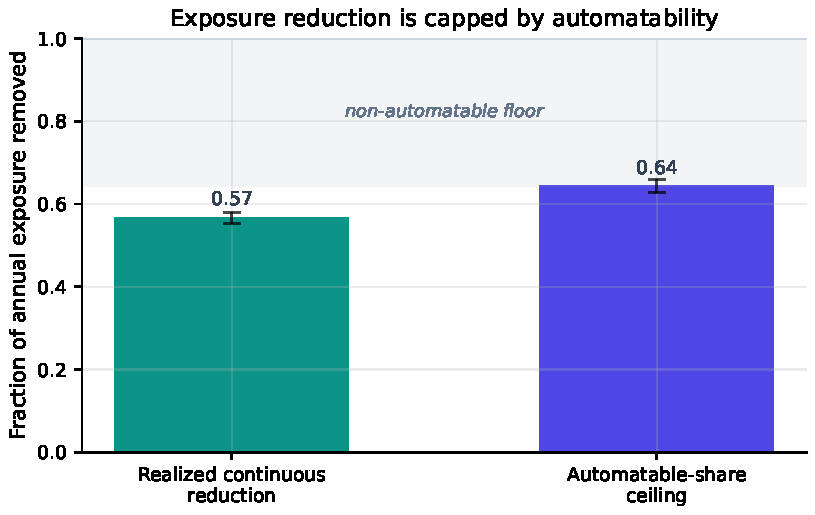
\includegraphics[width=\columnwidth]{fig1_ceiling.pdf}
\caption{The exposure reduction realized by continuous monitoring (left bar) sits below the ceiling
set by the automatable-exposure share (right bar); the gap between the ceiling and unity is the
floor formed by controls a machine cannot check.}\label{fig:ceiling}\end{figure}

\begin{figure}[t]\centering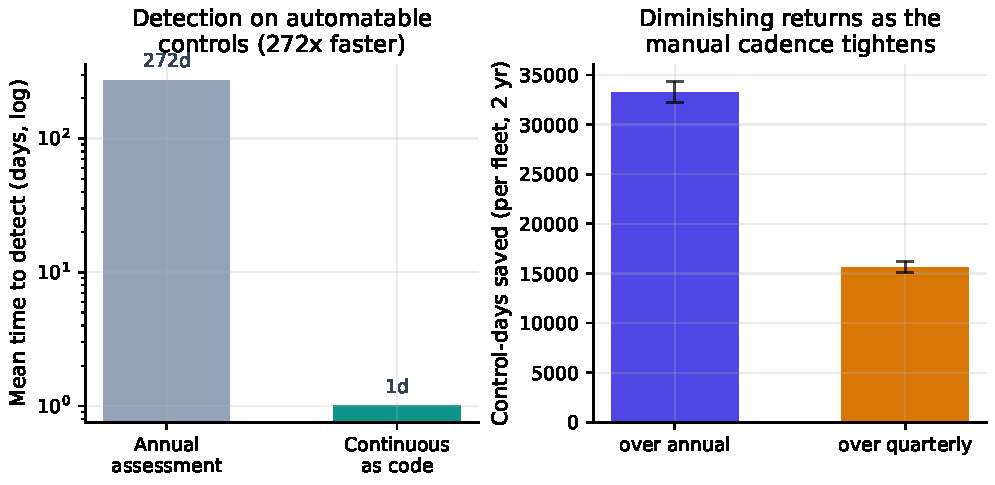
\includegraphics[width=\columnwidth]{fig2_mttd_cadence.pdf}
\caption{Left: mean time to detect on automatable controls falls 272-fold from annual assessment to
continuous monitoring. Right: the absolute control-days saved diminish as the manual cadence
tightens from annual to quarterly.}\label{fig:mttd}\end{figure}

\section{Theoretical Analysis}
\label{sec:theory}
The four empirical findings are not coincidences of the chosen constants; each is the visible face
of a structural relationship that the exposure decomposition makes explicit. This section derives
the automatability ceiling, the diminishing-returns relation, and the drift-concentration result in
closed form from the System Model, and then checks the closed form against the frozen numbers. The
framing mirrors the information-and-coverage view of a fundamental limit~\cite{cover2006elements}: detection speed is a channel, automatability
is the coverage of that channel, and no amount of channel quality can act on the part of the
catalog the channel does not reach.

\subsection{The exposure decomposition}
Write the exposure of a single drift event as the sum of the time it stays undetected and the fixed
remediation it then incurs. Summing over the drifts of control $i$ and then over controls, and
replacing the per-event latency by its mean, the system exposure under a monitoring regime is
\begin{equation}
\label{eq:decomp}
E \;=\; \sum_{i=1}^{N} \lambda_i \,\big( \bar d_i + \tau_r \big),
\end{equation}
where $\lambda_i$ is the expected number of detected drifts of control $i$ over the horizon,
$\bar d_i$ is its mean detection latency, and $\tau_r$ is the fixed remediation time. Equation
(\ref{eq:decomp}) is the mean-field form of the per-event sum in Eq.~(1): exposure is the product of
how often a control drifts and how long each drift persists, summed across the catalog. The
monitoring regime enters only through the latencies $\bar d_i$; the drift rates $\lambda_i$ and the
remediation $\tau_r$ are properties of the system and the response process, not of the detector.

\subsection{The automatability ceiling}
Partition the catalog into the automatable set $\mathcal{A} = \{ i : a_i = 1 \}$ and its complement.
Under continuous monitoring, an automatable control is evaluated on the one-day collection cadence,
so its latency falls toward the collection interval $c = 1$ day, while a non-automatable control
keeps the periodic latency $\bar d_i^{\,T}$ it had under the baseline cadence $T$. Decompose the
baseline (periodic) exposure into the part carried by automatable controls and the part carried by
the rest,
\begin{equation}
\label{eq:split}
E_{\text{per}} \;=\; \underbrace{\sum_{i \in \mathcal{A}} \lambda_i \big( \bar d_i^{\,T} + \tau_r \big)}_{E_{\mathcal{A}}^{\text{per}}}
\;+\; \underbrace{\sum_{i \notin \mathcal{A}} \lambda_i \big( \bar d_i^{\,T} + \tau_r \big)}_{E_{\bar{\mathcal{A}}}^{\text{per}}} .
\end{equation}
Continuous monitoring changes only the first sum and leaves the second untouched, so the exposure it
removes is
\begin{equation}
\label{eq:removed}
E_{\text{per}} - E_{\text{cont}} \;=\; \sum_{i \in \mathcal{A}} \lambda_i \big( \bar d_i^{\,T} - c \big) ,
\end{equation}
because the $\tau_r$ terms cancel and the latency of each automatable control drops from
$\bar d_i^{\,T}$ to $c$. The fractional reduction is therefore
\begin{equation}
\label{eq:R}
R \;=\; \frac{E_{\text{per}} - E_{\text{cont}}}{E_{\text{per}}}
\;=\; \frac{\sum_{i \in \mathcal{A}} \lambda_i \big( \bar d_i^{\,T} - c \big)}{E_{\text{per}}}.
\end{equation}
Now bound the numerator. For every automatable control $\lambda_i (\bar d_i^{\,T} - c) \le \lambda_i
(\bar d_i^{\,T} + \tau_r)$, because $c \ge 0$ and $\tau_r \ge 0$, so the numerator of
Eq.~(\ref{eq:R}) is at most $E_{\mathcal{A}}^{\text{per}}$. Dividing by $E_{\text{per}}$,
\begin{equation}
\label{eq:ceiling}
R \;\le\; \frac{E_{\mathcal{A}}^{\text{per}}}{E_{\text{per}}} \;\equiv\; C ,
\end{equation}
which is exactly the automatable-exposure share of Eq.~(3). Equation (\ref{eq:ceiling}) is the
\emph{automatability ceiling}: no matter how fast or how cheap the collection cadence becomes,
continuous monitoring cannot remove more than the share of baseline exposure that the automatable
controls carry, because the exposure of the un-automatable remainder $E_{\bar{\mathcal{A}}}^{\text{per}}$
is invariant under the detector. The floor on residual exposure is $1 - C$ of the baseline, and it is
a property of the catalog, not of the monitoring program.

The bound is tight only in the unreachable limit $c \to 0$ and $\tau_r \to 0$; at the model's
operating point the realized reduction sits strictly below $C$ by the residual that the automatable
controls themselves still carry. Substituting $\bar d_i^{\,T} - c = (\bar d_i^{\,T} + \tau_r) - (c +
\tau_r)$ into Eq.~(\ref{eq:R}) and writing $\rho$ for the exposure-weighted mean of $(c + \tau_r) /
(\bar d_i^{\,T} + \tau_r)$ over $\mathcal{A}$ gives the exact relation
\begin{equation}
\label{eq:gap}
R \;=\; C \,\big( 1 - \rho \big) ,
\end{equation}
so the ceiling gap $C - R = C\rho$ is the fraction of automatable exposure that the residual one-day
cadence and seven-day remediation leave in place. The gap is small but strictly positive precisely
because $c$ and $\tau_r$ are small relative to the periodic latency on automatable controls, not zero.

\subsection{Diminishing returns against the manual cadence}
The absolute benefit is the numerator of Eq.~(\ref{eq:R}), the control-days saved,
\begin{equation}
\label{eq:saved}
\Delta(T) \;=\; E_{\text{per}}(T) - E_{\text{cont}}(T) \;=\; \sum_{i \in \mathcal{A}} \lambda_i \big( \bar d_i^{\,T} - c \big).
\end{equation}
For a Poisson drift detected at the next assessment boundary of a periodic-$T$ regime, the mean
latency is increasing in $T$: a longer interval between assessments leaves a drift undetected
longer, so $\bar d_i^{\,T}$ grows with $T$ and $\bar d_i^{\,T'} \le \bar d_i^{\,T}$ whenever $T' \le
T$. Continuous monitoring drives the same automatable latencies to $c$ regardless of $T$.
Therefore, term by term in Eq.~(\ref{eq:saved}),
\begin{equation}
\label{eq:dimret}
\Delta(T') \;=\; \sum_{i \in \mathcal{A}} \lambda_i \big( \bar d_i^{\,T'} - c \big) \;\le\; \sum_{i \in \mathcal{A}} \lambda_i \big( \bar d_i^{\,T} - c \big) \;=\; \Delta(T)
\end{equation}
for $T' \le T$. The tighter the manual cadence, the smaller the absolute control-days continuous
monitoring can add, because the manual cadence has already removed part of the latency that
continuous monitoring would otherwise eliminate. The fractional reduction, by contrast, stays near
$C$ across cadences, because the denominator $E_{\text{per}}(T)$ shrinks with $T$ at nearly the same
rate as the numerator. Diminishing returns are therefore an absolute, not a fractional, phenomenon.

\subsection{Drift concentration}
Equation (\ref{eq:saved}) is a sum weighted by $\lambda_i$, so the controls that drift most often
dominate the saved exposure. Let the automatable controls be sorted by descending $\lambda_i$ and
let $\mathcal{Q}$ be the highest-drift quartile. Because the per-control saving $\lambda_i (\bar
d_i^{\,T} - c)$ is itself proportional to $\lambda_i$ (the latency factor $\bar d_i^{\,T} - c$
varies little across automatable controls under a common cadence), the share of $\Delta(T)$
captured by $\mathcal{Q}$ is approximately
\begin{equation}
\label{eq:concentration}
\frac{\sum_{i \in \mathcal{Q}} \lambda_i \big( \bar d_i^{\,T} - c \big)}{\sum_{i \in \mathcal{A}} \lambda_i \big( \bar d_i^{\,T} - c \big)} \;\approx\; \frac{\sum_{i \in \mathcal{Q}} \lambda_i}{\sum_{i \in \mathcal{A}} \lambda_i} .
\end{equation}
When the drift distribution is heavy-tailed, the right-hand side of Eq.~(\ref{eq:concentration})
is large even though $\mathcal{Q}$ is a quarter of the controls. In the model the rate is a
two-component mixture in which a 30\% technical stratum drifts at 6 per year and the remaining 70\%
at 0.5 per year, a twelve-fold ratio. The high-drift stratum thus carries a disproportionate share
of $\sum_i \lambda_i$, and because that stratum is also the most automatable, the highest-drift
quartile captures the large majority of the achievable reduction. Concentration follows from
heavy-tailedness alone and would survive any drift distribution with a comparable spread.

\subsection{Numerical verification against the frozen results}
The closed form must reproduce the frozen numbers, not merely point in their direction. The ceiling
of Eq.~(\ref{eq:ceiling}) is the automatable-exposure share, which the frozen results report as
$C = 0.6435$ ($[0.628, 0.660]$), and the realized fractional reduction of Eq.~(\ref{eq:R}) is
$R = 0.5669$ ($[0.553, 0.581]$). The inequality $R \le C$ holds with a gap of $C - R = 0.0766$, and
the gap is explained quantitatively by Eq.~(\ref{eq:gap}): the automatable controls still carry a
one-day collection cadence plus a seven-day remediation, an eight-day residual against a periodic
latency that on automatable controls averages 272 days before remediation, so the residual fraction
$\rho = (C - R)/C = 0.119$ is small and positive, exactly as the derivation requires. The ceiling
binds and is not exceeded; the realized reduction sits below it by the residual the automatable
controls cannot shed. The diminishing-returns inequality of Eq.~(\ref{eq:dimret}) is confirmed by
the frozen control-days saved, 33{,}266 against annual and 15{,}584 against quarterly, with
$\Delta(\text{quarterly}) < \Delta(\text{annual})$ by about 17{,}700 control-days. The concentration
relation of Eq.~(\ref{eq:concentration}) is confirmed by the frozen top-quartile capture of $0.786$
($[0.777, 0.796]$), well above a uniform-share expectation of one quarter. Each closed-form
statement matches the pre-registered numbers it predicts; where the match is approximate rather than
exact, as in Eq.~(\ref{eq:concentration}), it is stated as an approximation and the residual is
attributed to the mild variation of the latency factor across controls rather than asserted away.

\section{Robustness and Sensitivity}
\label{sec:robustness}
The headline numbers are means over 25 seeds; this section examines how they move across the manual
cadence and across the drift distribution, using only the frozen sweeps, and then asks what an
adversary can do with the residual the ceiling leaves in place.

\subsection{Sensitivity to the manual cadence}
Table~\ref{tab:cadence} reports the benefit of continuous monitoring against the two manual cadences
agencies actually run. The fractional reduction is nearly flat, from $0.567$ against annual to
$0.552$ against quarterly, because it tracks the automatable-exposure share $C$ and that share is a
property of the catalog rather than of the cadence. The absolute control-days saved, by contrast,
fall by more than half, from 33{,}266 to 15{,}584, exactly the diminishing-returns relation of
Eq.~(\ref{eq:dimret}): a quarterly baseline has already removed much of the latency that continuous
monitoring would otherwise eliminate, so the remaining headroom is smaller. The practical reading is
that the fractional case for automation is cadence-independent but the absolute case is strongest
where the manual baseline is weakest.

\begin{table}[t]
\centering
\caption{Sensitivity to the manual baseline cadence (mean over 25 seeds, 95\% BCa interval). The
fractional reduction tracks the automatable share and is nearly flat; the absolute control-days
saved diminish as the cadence tightens.}
\label{tab:cadence}
\footnotesize
\setlength{\tabcolsep}{4pt}
\adjustbox{max width=\columnwidth}{%
\begin{tabular}{@{}lcc@{}}
\toprule
Manual baseline & Fractional reduction $R$ & Control-days saved \\
\midrule
Annual ($T=365$)    & $0.567\ [0.553, 0.581]$ & $33{,}266\ [32{,}204, 34{,}387]$ \\
Quarterly ($T=90$)  & $0.552\ [0.540, 0.563]$ & $15{,}584\ [15{,}074, 16{,}211]$ \\
\bottomrule
\end{tabular}}
\end{table}

\subsection{Concentration across the drift distribution}
Table~\ref{tab:concentration} reports how much of the achievable reduction the highest-drift
quartile of controls captures, against the uniform-share benchmark of one quarter. Automating the
top-drift quartile alone realizes a fractional reduction of $0.446$ ($[0.435, 0.457]$), which is
$0.786$ ($[0.777, 0.796]$) of the $0.567$ reduction available from automating every automatable
control. A quarter of the controls thus delivers nearly four-fifths of the benefit, a more than
three-fold concentration over the uniform expectation, confirming Eq.~(\ref{eq:concentration}) on
the frozen sweep. The deployment ordering is immediate: instrument the high-drift quartile first.

\begin{table}[t]
\centering
\caption{Drift concentration: reduction captured by the highest-drift quartile of controls (mean
over 25 seeds, 95\% BCa interval), against the uniform-share benchmark.}
\label{tab:concentration}
\footnotesize
\setlength{\tabcolsep}{4pt}
\adjustbox{max width=\columnwidth}{%
\begin{tabular}{@{}lcc@{}}
\toprule
Automated subset & Fractional reduction $R$ & Share of full reduction \\
\midrule
Top-drift quartile     & $0.446\ [0.435, 0.457]$ & $0.786\ [0.777, 0.796]$ \\
All automatable controls & $0.567\ [0.553, 0.581]$ & $1.000$ \\
Uniform-share benchmark  & n/a & $0.250$ \\
\bottomrule
\end{tabular}}
\end{table}

\subsection{Adversarial robustness of the residual}
The ceiling has an adversarial reading that the means conceal. The automatability ceiling guarantees
a residual exposure of $1 - C \approx 0.357$ of baseline that no detection speed can lower, and that
residual lives entirely in the un-automatable controls, the policy, documentation, and physical
controls that a machine cannot check. An adversary who understands the program will not attack the
instrumented controls, where a drift is caught within a day; the adversary will concentrate risk in the
un-automatable floor, where detection still runs on the periodic cadence $T$. By moving its activity
into the $1 - C$ share, an adversary defeats the automation program without ever tripping a
continuous check, because the program has no reach there by construction. The same orthogonal-signal
logic that makes a layered defense robust works in reverse here: an automation program that is
strong on exactly one axis, machine-checkability, is blind on the complementary axis, and a
strategic adversary will choose the blind axis. The residual must therefore be managed by other
means, a tighter manual assessment cadence on the specific high-impact policy and physical controls,
independent attestation, or human review keyed to change windows, rather than treated as acceptable
because the automatable controls are well covered. The ceiling is not only a limit on the benefit;
it is a map of where an adversary will go.

\section{Discussion}
The two benefits of compliance as code point in different directions, and conflating them produces
the optimism that this study is designed to puncture. Detection latency on automatable controls
collapses by a factor of 272; an agency that measures success by how fast it catches a disabled
audit log will see a transformative improvement. But the quantity that an authorization decision
turns on is exposure, the total control-days a system spends out of compliance, and exposure is
bounded by automatability. A reduction of 0.567 against an annual baseline is large and worth
pursuing, but it is closer to half than to the near-elimination that latency figures suggest, and
it cannot be pushed past the 0.643 ceiling by any improvement in collection speed. The right
program metric is the automatable-exposure share, not the detection-latency reduction.

The concentration result turns this into an actionable ordering. Because the top-drift quartile
captures nearly four-fifths of the achievable reduction, an agency should instrument its
high-drift, high-automatability technical controls first, the logging, certificate, configuration,
and access controls, and expect rapidly diminishing marginal returns thereafter. The diminishing-returns
result against cadence sharpens the business case: the gain from automation is largest for an
organization still assessing annually and roughly halves for one already on a quarterly cycle, so
the investment is most justified where the manual baseline is weakest.

Three deployment rules follow directly. First, size expectations to the automatable-exposure share,
not to detection latency, when projecting the compliance-exposure benefit of an
automation program. Second, sequence the rollout by drift frequency, because the high-drift
quartile dominates the return. Third, treat the un-automatable remainder as an irreducible
residual to be managed by other means, such as a tighter manual cadence on the specific
high-impact policy and physical controls, rather than as a target for automation.

\section{Threats to Validity}
\emph{Construct validity.} The model abstracts compliance drift as a Poisson process with a fixed
remediation time. Real drift may be bursty, correlated across controls (a single misconfigured
deployment can trip several controls at once), or seasonal around change windows, and remediation
time varies with the control and the team. These would shift absolute exposure values but not the
structural relationships: an automatability ceiling exists whenever any control is un-automatable,
and concentration follows from any heavy-tailed drift-rate distribution.

\emph{Internal validity.} Because the study is pre-registered and the evaluation seeds were
inspected only once, the reported numbers are not the product of analytic search. The development
of the model used separate seeds, and no distribution was tuned to clear a threshold. The
mechanical evaluation script computes each verdict from the frozen data with no hand-set value.

\emph{External validity.} The catalog size, the drift-rate mixture, and the automatability
probabilities are documented priors, not measurements from any agency, so the absolute magnitudes
(272 days, 33{,}266 control-days) should be read as illustrative of the model rather than as field
estimates. The comparative findings, the ceiling, the diminishing returns, and the concentration,
depend on the qualitative structure of the model rather than on the specific constants, and we
expect them to transfer. Calibrating the drift and automatability distributions against a real
control catalog and assessment record is the natural next step and would convert the illustrative
magnitudes into estimates.

\emph{Statistical validity.} Intervals are BCa bootstrap intervals over 25 seeds, appropriate for
the small-sample, possibly skewed statistics reported here; we use interval non-overlap rather than
significance testing throughout, avoiding the multiple-comparison pitfalls of repeated $p$-values.

\section{Conclusion}
Continuous automated evidence collection is transformative for detection latency on the controls it
can reach, turning months into a day, but the program-level benefit is governed by two facts that
the latency figure hides. A substantial share of controls cannot be machine-checked and sets a hard
floor on exposure, and exposure is dominated by the high-drift technical controls, which are also
the most automatable. In a pre-registered simulation, continuous monitoring cut detection latency
272-fold on automatable controls, removed 0.567 of annual exposure against a binding ceiling of
0.643, showed diminishing returns as the manual cadence tightened, and concentrated nearly
four-fifths of its value in the highest-drift quartile of controls. The deployment guidance is
correspondingly concrete: instrument the high-drift automatable controls first, size expectations
to the automatable-exposure share, and manage the un-automatable remainder as a residual rather
than a target. Calibrating the model against a real control catalog is the next step toward turning
these structural findings into field estimates.

% Generated by IEEEtran.bst, version: 1.14 (2015/08/26)
\begin{thebibliography}{10}
\providecommand{\url}[1]{#1}
\csname url@samestyle\endcsname
\providecommand{\newblock}{\relax}
\providecommand{\bibinfo}[2]{#2}
\providecommand{\BIBentrySTDinterwordspacing}{\spaceskip=0pt\relax}
\providecommand{\BIBentryALTinterwordstretchfactor}{4}
\providecommand{\BIBentryALTinterwordspacing}{\spaceskip=\fontdimen2\font plus
\BIBentryALTinterwordstretchfactor\fontdimen3\font minus
  \fontdimen4\font\relax}
\providecommand{\BIBforeignlanguage}[2]{{%
\expandafter\ifx\csname l@#1\endcsname\relax
\typeout{** WARNING: IEEEtran.bst: No hyphenation pattern has been}%
\typeout{** loaded for the language `#1'. Using the pattern for}%
\typeout{** the default language instead.}%
\else
\language=\csname l@#1\endcsname
\fi
#2}}
\providecommand{\BIBdecl}{\relax}
\BIBdecl

\bibitem{nist80053}
{Joint Task Force}, ``Security and privacy controls for information systems and
  organizations,'' National Institute of Standards and Technology, Tech. Rep.
  NIST Special Publication 800-53 Rev. 5, 2020.

\bibitem{nist80137}
K.~Dempsey, N.~S. Chawla, A.~Johnson, R.~Johnston, A.~C. Jones, A.~Orebaugh,
  M.~Scholl, and K.~Stine, ``Information security continuous monitoring (iscm)
  for federal information systems and organizations,'' National Institute of
  Standards and Technology, Tech. Rep. NIST Special Publication 800-137, 2011.

\bibitem{nist80137a}
K.~Dempsey, V.~Pillitteri, C.~Baer, R.~Niemeyer, R.~Rudman, and S.~Urban,
  ``Assessing information security continuous monitoring (iscm) programs:
  Developing an iscm program assessment,'' National Institute of Standards and
  Technology, Tech. Rep. NIST Special Publication 800-137A, 2020.

\bibitem{oscal}
{National Institute of Standards and Technology}, ``Open security controls
  assessment language ({OSCAL}),'' \url{https://pages.nist.gov/OSCAL/}, 2026,
  nIST CSRC project; accessed 2026-06-20.

\bibitem{opa}
{Open Policy Agent Project (Cloud Native Computing Foundation)}, ``Open policy
  agent: Policy-based control for cloud native environments,''
  \url{https://www.openpolicyagent.org/docs}, 2026, graduated CNCF project;
  accessed 2026-06-20.

\bibitem{powershelldsc}
{Microsoft}, ``Powershell desired state configuration ({DSC}),''
  \url{https://learn.microsoft.com/powershell/dsc/overview}, 2026, accessed
  2026-06-20.

\bibitem{efron1987bca}
B.~Efron, ``Better bootstrap confidence intervals,'' \emph{Journal of the
  American Statistical Association}, vol.~82, no. 397, pp. 171-185, 1987.

\bibitem{efron1994introduction}
B.~Efron and R.~J. Tibshirani, \emph{An Introduction to the Bootstrap}.\hskip
  1em plus 0.5em minus 0.4em\relax Chapman \& Hall/CRC, 1994.

\bibitem{wohlin2012experimentation}
C.~Wohlin, P.~Runeson, M.~H{\"o}st, M.~C. Ohlsson, B.~Regnell, and
  A.~Wessl{\'e}n, \emph{Experimentation in Software Engineering}.\hskip 1em
  plus 0.5em minus 0.4em\relax Springer, 2012.

\bibitem{fips199}
{National Institute of Standards and Technology}, ``Standards for security
  categorization of federal information and information systems,'' U.S.
  Department of Commerce, Tech. Rep. FIPS PUB 199, 2004.

\bibitem{nist80060}
K.~Stine, R.~Kissel, W.~C. Barker, J.~Fahlsing, and J.~Gulick, ``Guide for
  mapping types of information and information systems to security
  categories,'' National Institute of Standards and Technology, Tech. Rep. NIST
  Special Publication 800-60 Rev. 1, 2008.

\bibitem{rahman2019seven}
A.~Rahman, C.~Parnin, and L.~Williams, ``The seven sins: Security smells in
  infrastructure as code scripts,'' in \emph{Proceedings of the 41st
  International Conference on Software Engineering (ICSE)}, 2019, pp. 164-175.

\bibitem{rahman2021different}
A.~Rahman and L.~Williams, ``Different kind of smells: Security smells in
  infrastructure as code scripts,'' \emph{IEEE Security \& Privacy}, vol.~19,
  no.~3, pp. 33-41, 2021.

\bibitem{kephart2003vision}
J.~O. Kephart and D.~M. Chess, ``The vision of autonomic computing,''
  \emph{IEEE Computer}, vol.~36, no.~1, pp. 41-50, 2003.

\bibitem{nist2022sp80040r4}
{National Institute of Standards and Technology}, ``Guide to enterprise patch
  management planning: Preventive maintenance for technology,'' National
  Institute of Standards and Technology, Tech. Rep. NIST Special Publication
  800-40 Rev. 4, 2022.

\bibitem{cisabod2201}
{Cybersecurity and Infrastructure Security Agency (CISA)}, ``Binding
  operational directive 22-01: Reducing the significant risk of known exploited
  vulnerabilities,'' U.S. Department of Homeland Security, Tech. Rep., Nov.
  2021,
  \url{https://www.cisa.gov/news-events/directives/bod-22-01-reducing-significant-risk-known-exploited-vulnerabilities}.

\bibitem{cisabod2301}
{Cybersecurity and Infrastructure Security Agency (CISA)}, ``Binding
  operational directive 23-01: Improving asset visibility and vulnerability
  detection on federal networks,'' U.S. Department of Homeland Security, Tech.
  Rep., Oct. 2022,
  \url{https://www.cisa.gov/news-events/directives/bod-23-01-improving-asset-visibility-and-vulnerability-detection-federal-networks}.

\bibitem{verizon2026dbir}
{Verizon}, ``2026 data breach investigations report ({DBIR}),'' Verizon
  Business, Tech. Rep., 2026,
  \url{https://www.verizon.com/business/resources/reports/dbir/}.

\bibitem{paper4hygieneprio}
H.~Malla, ``{HygienePrio}: Cyber-hygiene signal augmentation for
  {EPSS}-weighted vulnerability prioritization,''
  \url{https://github.com/Harshavardhanmalla-Labs/research-papers/tree/main/paper4},
  2026, companion paper; source, code, and frozen results in the same
  repository.

\bibitem{paper1vulnprio}
H.~Malla, ``Context-aware vulnerability prioritization for government endpoint
  fleets,''
  \url{https://github.com/Harshavardhanmalla-Labs/research-papers/tree/main/paper1},
  2026, companion paper; source, code, and frozen results in the same
  repository.

\bibitem{cover2006elements}
T.~M. Cover and J.~A. Thomas, \emph{Elements of Information Theory},
  2nd~ed.\hskip 1em plus 0.5em minus 0.4em\relax Wiley, 2006.

\end{thebibliography}

\end{document}
